\documentclass[12pt,a4paper]{report}

\usepackage[T1]{fontenc}
\usepackage[utf8]{inputenc}
\usepackage[french]{babel}
\title{Rapport de stage\\
\large Réecriture et optimisation de progiciels de python dans le langage Golang}
\author{Quentin Agneray}
\date{\today}

\usepackage{hyperref}
\usepackage{graphicx}
\usepackage{fancyhdr}
\pagestyle{fancy}

\usepackage{color}
    \definecolor{lightgray}{rgb}{0.95, 0.95, 0.95}
    \definecolor{darkgray}{rgb}{0.4, 0.4, 0.4}
    \definecolor{purple}{rgb}{0.65, 0.12, 0.82}
    \definecolor{ocherCode}{rgb}{1, 0.5, 0} % #FF7F00 -> rgb(239, 169, 0)
    \definecolor{blueCode}{rgb}{0, 0, 0.93} % #0000EE -> rgb(0, 0, 238)
    \definecolor{greenCode}{rgb}{0, 0.6, 0} % #009900 -> rgb(0, 153, 0)
    
\usepackage{upquote}

\usepackage{listings}
\usepackage{listings-golang}
\lstdefinelanguage{HTML5}{
    sensitive=true,
    keywords={%
    % JavaScript
    typeof, new, true, false, catch, function, return, null, catch, switch, var, if, in, while, do, else, case, break,
    % HTML
    html, title, meta, style, head, body, script, canvas,
    % CSS
    border:, transform:, -moz-transform:, transition-duration:, transition-property:,
    transition-timing-function:
    },
    % http://texblog.org/tag/otherkeywords/
    otherkeywords={<, >, \/},   
    ndkeywords={class, export, boolean, throw, implements, import, this},   
    comment=[l]{//},
    % morecomment=[s][keywordstyle]{<}{>},  
    morecomment=[s]{/*}{*/},
    morecomment=[s]{<!}{>},
    morestring=[b]',
    morestring=[b]",    
    alsoletter={-},
    alsodigit={:}
}

\lstdefinestyle{Golang}{
	frame=single,
    basicstyle=\footnotesize,
    keywordstyle=\color{red},
    numbers=left,
    numbersep=5pt,
    showstringspaces=false, 
    stringstyle=\color{blue},
    tabsize=4,
    language=Golang % this is it !
}

\lstdefinestyle{HTML5}{
	% Basic design
    backgroundcolor=\color{lightgray},
    basicstyle={\small\ttfamily},   
    frame=single,
    % Line numbers
    xleftmargin={0.75cm},
    numbers=left,
    stepnumber=1,
    firstnumber=1,
    numberfirstline=true,
    % Code design
    identifierstyle=\color{black},
    keywordstyle=\color{blue}\bfseries,
    ndkeywordstyle=\color{greenCode}\bfseries,
    stringstyle=\color{ocherCode}\ttfamily,
    commentstyle=\color{darkgray}\ttfamily,
    % Code
    language={HTML5},
    tabsize=2,
    showtabs=false,
    showspaces=false,
    showstringspaces=false,
    extendedchars=true,
    breaklines=true
}


\usepackage{afterpage}

\usepackage{titlesec, blindtext}
\definecolor{gray75}{gray}{0.75}
\newcommand{\hsp}{\hspace{20pt}}
\titleformat{\chapter}[hang]{\Huge\bfseries}{\thechapter\hsp\textcolor{gray75}{|}\hsp}{0pt}{\Huge\bfseries}

\newcommand\blankpage{%
    \null
    \thispagestyle{empty}%
    \addtocounter{page}{-1}%
    \newpage}
    
\renewcommand{\thechapter}{\Roman{chapter}}
\renewcommand{\thesubsection}{\thesection.\alph{subsection}}
  
\begin{document}

\maketitle

\afterpage{\blankpage}

\tableofcontents
\listoffigures
\chapter[Remerciements]{Remerciements}
Je tiens dans un premier temps à remercier tous les membres de l'entreprise que j'ai côtoyé pendant ce stage, en particulier monsieur Michel Dewintre gérant de l'agence qui a eu l'amabilité de m'accueillir pendant trois mois.\\

Je remercie également les membres du jury qui ont accepté de présider lors de ma soutenance.\\

Je remercie mon responsable de formation ainsi que mon tuteur Monsieur Eric Timmerman et l'ensemble des professeurs et intervenants qui m'ont suivi pendant mon parcours d'étudiant en DUT Informatique.
\newpage
\chapter[Introduction]{Introduction}
Le rapport que je vais vous exposer a été fait dans le cadre de ma deuxième
année d'études en tant qu'étudiant en Diplômes Universitaires de Technologie
(DUT) ayant pour spécialité l'informatique.\\

L'objectif de se stage est de mettre à profit les compétences que j'ai acquises dans le cadre de mes études, d'apprendre de nouvelle choses dans un environnement professionnel.\\

 Le stage que j'ai effectué a eu une durée d'environ trois mois du 14 mai 2018 au 3 aout 2018. Ce stage a été effectué au sein de l'agence de voyage Alloa située au 72 Rue Léon Gambetta à Lille. J'ai choisi cette entreprise car je voulais apprendre un nouveau langage, le Golang(Go) ainsi que d'autre technologies comme GopherJS, gRPC, Protocol Buffers, postgreSQL, Bootstraps.\\
 
 Ma mission lors de ce stage a été de réécrire et d'optimiser les progiciels de l'agence écrit en python dans le langage Golang.\\
 
 Tous d'abord je vais vous faire une présentation de l'entreprise Alloa, de ses acteurs ainsi que  l'environnement de travail (logiciels utilisés, répartition des tâches,...). Ensuite je vous parlerai de l'avancement de mes différentes missions, de la partie développement ainsi que de l'analyse de code. Pour finir, je vous exposerai les différentes compétences que j'ai acquis qui pourrons mettre utile pour mon futur emploi.
\newpage
\chapter[Présentation]{Présentation de l'entreprise}
\section{Alloa Voyages}

\subsection{L'agence de voyage}

L'entreprise Alloa Voyages est située à Lille à l'adresse 72, rue Léon Gambetta.
L'agence à été créer en 1981 et à comme nom Apolinea Club, c'est une association. En 1983 l'agence  adopte le statut juridique de la SARL et se renomme en Amphitrite. La devise de l'agence est ne me demandé pas la lune je ne fait que le monde.\\

L'entreprise n'a pas de clientèle  principale et travail avec les entreprises, les particuliers ainsi que les familles. L'agence ne possède pas de concurrent direct dans son domaine d'activité et propose des voyages sur mesure à ces clients.
\subsection{L'agence et le domaine de l'informatique}
L'agence Alloa est familiarisé depuis longtemps avec l'informatique. L'entreprise à créer le premier programme d'agence de voyage pour la comptabilité d'abord sur minitel puis sur internet. La licence choisie fut propriétaire puis open source.\\

 Elle possède ces propre serveurs et utilise comme plateforme d'orchestration de containers Kubernetes. Les serveurs sont regroupés et forme une grappe de serveur ou cluster\footnote{un cluster consiste à associer divers noeuds afin de les faire travailler ensemble en partageant des ressources communes}
Le système d'exploitation utilisé sur les serveurs  est Debian car le système d'exploitation est fiable et accessible.\\



\section{Technologies utilisées}
\subsection{Golang et GopherJS}
Golang est un langage de programmation open source compilé proche du C ou du Pascal  développé en interne dans les laboratoires de Google à partir de 2007. Ce langage à été dévelopé par Robert Griesemer qui a contribué au compilateur JavaScript V8 par Rob Pike qui a travaillé sur l'UTF-8 et Kenneth Lane Thompson qui a travaillé sur l'écriture du système Unix.\\

Quelques différences entre le Golang et le langage Java que j'ai appris lors de mon cursus. Le Golang permet de retourner plusieurs valeurs contrairement au Java. Autre différence en Golang nous utilisons des structures et non des classes. Pour finir en golang pour rendre une variable visible à l'extérieur du package nous mettons la première lettre de la variable en capital et n'utilisons pas des mots clefs comme public, private et protected.\\

GopherJS est un transpileur\footnote{traduit un code source dans un langage de programmation et le compile dans un autre langage} développé par Richard Musiol à partir d'aout 2013 qui permet de convertir du code Golang en code JavaScript exécutable sur tous les navigateurs.\\



\newpage
Voici un exemple de code écrit en GopherJS et son équivalent écrit en javascript inclut dans une page html à l'aide de balise <script>...</script>\\
\lstset{style=Golang}
\begin{lstlisting}
package main

import "fmt"
import "github.com/gopherjs/gopherjs/js"

func main() {
    js.Global.Call("alert","hello world")
}
\end{lstlisting}

\lstset{style=HTML5}
\begin{lstlisting}
<!DOCTYPE html>
<html>
<body>
<script>
function maFonction() {
	alert("hello world");
}
</script>
<body>
</html>
\end{lstlisting}


\subsection{gRPC et Protocol Buffers}
gRPC est un framework RPC (Remote Procedure Call) développé par Google. RPC est un protocole IP qui permet de développer des applications client-serveur. RPC ce situe dans la couche 5 dite Session du modèle OSI (Open Systems Interconnection).\\

Protocol Buffers est un système de sérialisation de données\footnote{processus de conversion d'un objet en un flux d'octets pour stocker l'objet ou le transmettre}. Il est utilisé  avec le langage Java et le Golang qui ne supporte pas très bien le JSON qui est un autre système de sérialisation de données.\\


\newpage
Voici un exemple de fichier protobuf:
\lstset{style=Golang}
\begin{lstlisting}
package web;


import "github.com/johanbrandhorst/protobuf/proto/gopherjs.proto"

message Destination {
  string lib = 1;
  string uuid = 2;
  repeated Pays pays = 3;
}
\end{lstlisting}
\subsection{PostgreSQL}
PostgreSQL est un système de bases de données relationnelles objet développé à l'université de Berkeley en Californie en 1986 sous le nom de POSTGRES puis PostegreSQL  à partir de 1996. Pour administrer notre base de donnée nous avons  utilisé pgAdmin qui est un outil pour PostgreSQL. Ce logiciel m'a permis de tester mes requêtes sur la base de donnée et de voir le contenue des tables. Pour finir j'ai travaillé sur pgModeler pour visualiser le MCD (Modèle Conceptuel de Données) , ce qui m'a permis de voir les tables et les différents liens, relations entre celles-ci.



\subsection{Bootstrap}
Bootstrap est un framework web côté client \textit{frontend}. Bootstrap inclut de l'HTML du CSS ainsi que du JavaScript. L'avantage de Bootstrap est qu'il est facile à utiliser et est compatible avec de nombreux navigateur. L'autre avantage majeur et qu'il s'adapte au téléphone, tablettes ainsi que pour les moniteurs d'ordinateur de bureau. Ceci s'appelle le RWD (Responsive Web Design) et ce concept vient du web designer Ethan Marcotte.





\chapter[Missions]{Missions}

\section{Présentation et Organisation}
Mes missions lors de ce stage on été de réécrire et d'optimiser les progiciels de l'agence de Python en Golang. Le choix du Golang pour la réécriture des progiciels n'a pas été la seul option envisagée. En premier lieu des tests on été fait avec Angular et Vue.js.\\ 

Angular est un framework coté client qui permet de construire des applications mobiles et web. Angular utilise Typescript, qui est un langage qui permet le développement d'applications écrites en JavaScript. Vue.js quand à lui est un framework javaScript pour créer des interfaces utilisateurs.\\

Nous n'avons pas retenue cette solution car trop lourde. Nous avons préféré utiliser le Golang qui répond plus à notre besoin. En effet le Golang prend en charge des machines multi-coeur et permet d'être déployer facilement avec Kubernetes que nous utilisons. Golang peut être utiliser pour construire un CMS(Content Management System) qui permet de gérer des sites web.\\

Pour mener à bien les différents projets nous avons utilisé Git qui est un logiciel de gestion de version et Gitlab qui nous a permis de pouvoir gérer nos dépôts Git. Sur Gitlab nous avons utilisé un outil qui s'appelle une issue qui permet de suivre l'évolution du projet avec la liste des tâches à effectuer et leur avancement avec un système de To Do (A Faire) , Doing (Faire) et Done (Terminé). Système similaire à celui que j'ai utilisé lors des projets Agile fait lors de mon cursus.\\

Comme logiciel de communication nous nous somme servie de pidgin qui est un logiciel de messagerie instantanée. Ce logiciel nous a permis de nous envoyer de la documentation technique et du code.\\
\newpage
Au niveau de l'organisation, nous nous somme organisé de la manière  suivante. J'ai tous d'abord travaillé sur la réécriture du logiciel Hyooper côté Back-End (Serveur)  avec l'aide d'un autre stagiaire Valerian. Celui-ci m'a expliqué le projet et son organisation hiérarchique (packages, comment compiler le projet, les branches sur Git, ...). Par la suite je me suis occupé du côté Front-End (HTML,CSS,JavaScript,GopherJS) pour prendre la place d'un stagiaire Quentin qui à commencé le site commercial de l'agence. Pour finir j'ai travaillé sur le site commercial de l'agence côté Back-End avec Quentin  et Front-End avec Maxime, stagiaire que j'ai du former.\\

Pour ce qui est du suivi du projet nous discutions entre nous et avec monsieur Dewintre aussi souvent que possible pour voir les différentes difficultés rencontrées et des améliorations éventuelle à apporter.\\

Au niveau de mon organisation personnel pour mon travail, j'ai beaucoup travaillé à l'aide d'un papier et d'un crayon. Cela m'a permis de prendre des notes et de coucher par écrit mes idées sur comment résoudre certaine difficultés et consigner les bugs que j'ai rencontré pour pouvoir les remonter.\\

\section{Hyooper}

Hyooper est un progiciel de gestion globale de l'agence de voyage. Ce logiciel à pour but de faciliter l'ajout, la suppression et la modification d'informations sur des composantes d'un voyage par exemple comme  une destination, un hébergement, un circuit touristique ... Mais pas seulement il permet également de pouvoir gérer tous ce qui concerne le marketing, la direction , les sous traitant ...\\

\begin{figure}[!h]
\centerline{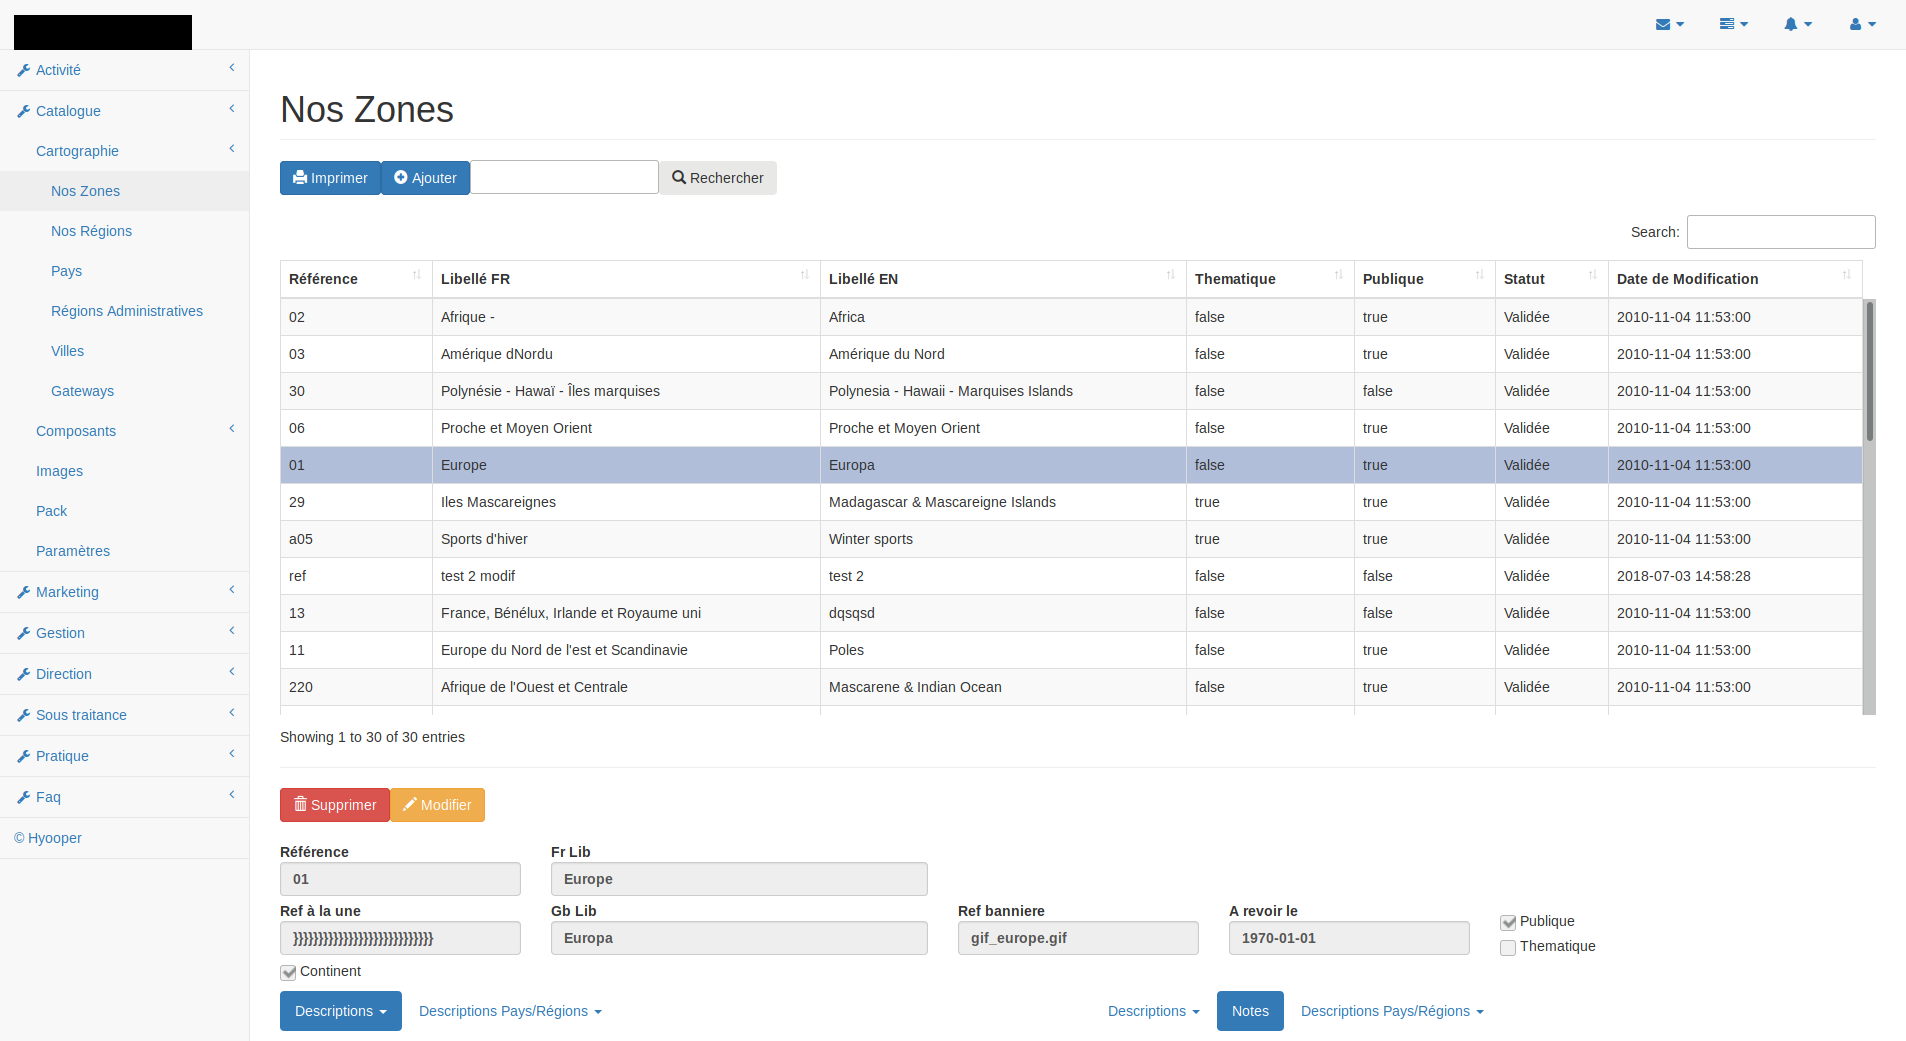
\includegraphics[scale=0.3]{hyooper.png}}
\caption{logiciel hyooper module Nos Zones (Destinations)}
\label{image_hyooper}
\end{figure}



Le travail que j'ai effectué à été de créer des "modules" sur la composante d'un voyage comme les villes , les régions, les pays ... Mon but à été de créer des fonctions pour récupérer des informations sur une ville par exemple en faisant une requête de type SELECT sur la base de donnée. J'ai également créer des structures pour définir par exemple qu'est ce qu'une destination et qu'une destination ce compose d'un Uuid(Universally Unique IDentifier) , d'une référence, d'un libellé  français et anglais ... Pour obtenir les informations concernant le contenue des modules (tables), j'ai utilisé PgModeler pour voir les données à récupérer ainsi que leur types(chaine de caractères , entier, booléen , date ,...).\\

Pour ce qui est du côté client, je me suis assuré de la mise en page ainsi que de la  récupération des données et de leur ajout dans le fichier HTML en utilisant GopherJS. Pour la mise en page du site nous avons utiliser Bootstrap et en particulier SB Admin 2 qui est un template\footnote{un template est un modèle pour l'architecture du design d'une page }. La création des zones de texte pour l'affichage de la description d'un module c'est fait grâce à l'API(Application Programming Interface) Quill.

\section{Site Commercial}



\end{document}